% Self-contained LaTeX TikZ causal DAG template.
% Compile: pdflatex causal_dag.tex
% Roles: treatment / outcome / confound / mediator / instrument / latent
\documentclass[border=10pt]{standalone}
\usepackage[utf8]{inputenc}
\usepackage{tikz}
\usetikzlibrary{positioning, arrows.meta, shapes.geometric, calc, decorations.pathreplacing}

\begin{document}
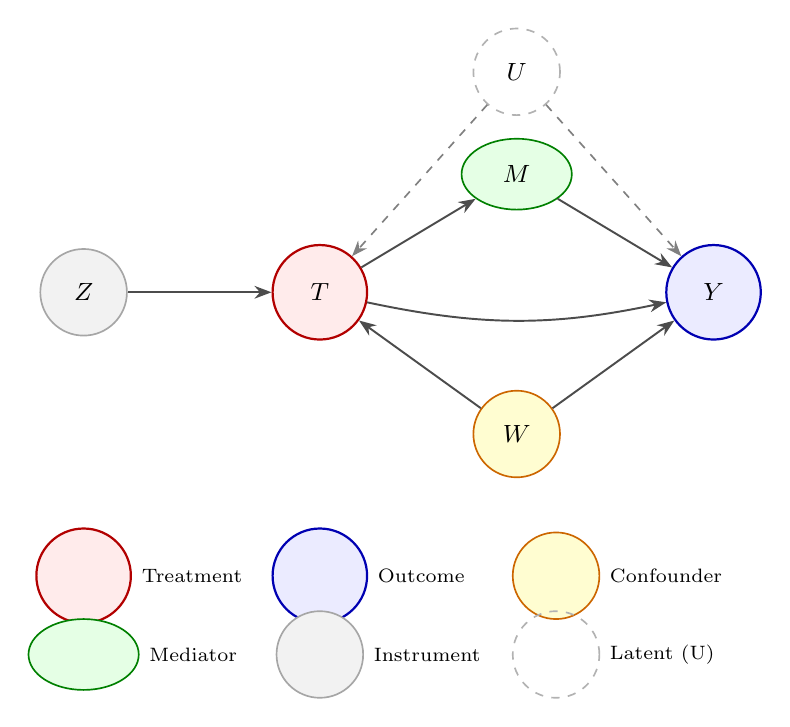
\begin{tikzpicture}[
    >=Stealth,
    node distance=18mm and 24mm,
    every node/.style={font=\small},
    treat/.style={circle, draw=red!70!black, fill=red!8, line width=0.8pt,
                  minimum size=12mm, inner sep=1pt},
    outcome/.style={circle, draw=blue!70!black, fill=blue!8, line width=0.8pt,
                    minimum size=12mm, inner sep=1pt},
    conf/.style={circle, draw=orange!80!black, fill=yellow!18, line width=0.6pt,
                 minimum size=11mm, inner sep=1pt},
    med/.style={ellipse, draw=green!50!black, fill=green!10, line width=0.6pt,
                minimum width=14mm, minimum height=9mm, inner sep=1pt},
    iv/.style={circle, draw=gray!70, fill=gray!10, line width=0.6pt,
               minimum size=11mm, inner sep=1pt},
    latent/.style={circle, draw=gray!60, dashed, line width=0.6pt,
                   minimum size=11mm, inner sep=1pt},
    edge/.style={->, line width=0.7pt, draw=black!70},
    dashedge/.style={->, line width=0.6pt, draw=gray, dashed},
]

% Nodes
\node[iv]      (Z) at (0, 0)         {$Z$};
\node[treat]   (T) at (3, 0)         {$T$};
\node[med]     (M) at (5.5, 1.5)     {$M$};
\node[outcome] (Y) at (8, 0)         {$Y$};
\node[conf]    (W) at (5.5, -1.8)    {$W$};
\node[latent]  (U) at (5.5, 2.8)     {$U$};

% Edges
\draw[edge] (Z) -- (T);
\draw[edge] (T) -- (M);
\draw[edge] (M) -- (Y);
\draw[edge] (T) to[bend right=12] (Y);
\draw[edge] (W) -- (T);
\draw[edge] (W) -- (Y);
\draw[dashedge] (U) -- (T);
\draw[dashedge] (U) -- (Y);

% Legend (optional, comment out if unwanted)
\begin{scope}[shift={(0, -3.6)}, every node/.style={font=\scriptsize}]
  \node[treat,   label=right:{Treatment}]   at (0, 0)   {};
  \node[outcome, label=right:{Outcome}]     at (3, 0)   {};
  \node[conf,    label=right:{Confounder}]  at (6, 0)   {};
  \node[med,     label=right:{Mediator}]    at (0, -1)  {};
  \node[iv,      label=right:{Instrument}]  at (3, -1)  {};
  \node[latent,  label=right:{Latent (U)}]  at (6, -1)  {};
\end{scope}

\end{tikzpicture}
\end{document}
